\documentclass[12pt]{article}
\usepackage[table]{xcolor}
\usepackage{tabularx}
\usepackage{graphicx}
\usepackage{hyperref}
\usepackage{verbatim}
\usepackage{geometry}
\usepackage{ulem}
\usepackage[official]{eurosym}
\usepackage{tikz}
\usetikzlibrary{arrows,backgrounds,calc}
\usepackage{pgfplots}
\pgfplotsset{compat = newest}
\usetikzlibrary{fit}
\newcommand\addvmargin[1]{
\usetikzlibrary{arrows}
\node[fit=(current bounding box),inner ysep=#1,inner xsep=0]{};}
\usepackage{cancel}
\usepackage{fontspec}
\usepackage{array}  
\geometry{a4paper, top=2cm, left=2cm, right=2cm, bottom=2cm, headsep=1cm}
\usepackage{tabu}
\usepackage{pst-node}
\usepackage{colortbl}
\usepackage{array}
\usepackage{german}
\setlength\parindent{0pt}
\newcolumntype{?}{!{\vrule width 1pt}}
\usepackage{makecell}
\renewcommand{\arraystretch}{2.5}
\usepackage{pbox}
\usepackage{amssymb}
\usepackage{amsmath}
\usepackage{booktabs}
\newcolumntype{L}[1]{>{\raggedright\let\newline\\\arraybackslash\hspace{0pt}}m{#1}}
\newcolumntype{C}[1]{>{\centering\let\newline\\\arraybackslash\hspace{0pt}}m{#1}}
\newcolumntype{R}[1]{>{\raggedleft\let\newline\\\arraybackslash\hspace{0pt}}m{#1}}
\begin{document}
\rightline{Datum: 11.01.2023}
\centerline{{\Large Hausaufgabentag}} 
\vspace{1cm}
\noindent Fülle die Tabellen aus\\


\begin{tabularx}{\textwidth}{|C{1.0cm}|X|C{1.0cm}|X|}
\arrayrulecolor{black}\hline
a)&\tikzstyle{background grid}=[draw, black!15,step=.5cm]
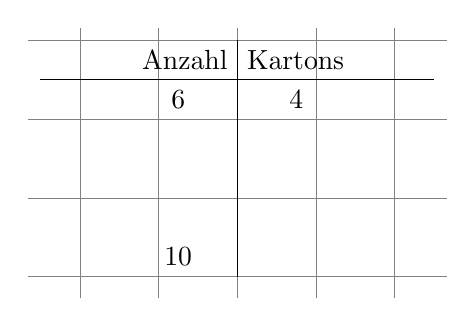
\begin{tikzpicture}[show background grid]
\draw[black] (0cm,0cm) -- (0cm,-3cm); 
\draw[black] (-2.5 cm,-0.5cm) -- (2.5cm,-0.5cm); 
\node[left] at (0 cm,-0.25cm) {Anzahl};
\node[right] at (0 cm,-0.255cm) {Kartons};
\node[circle] (1) at (-0.75 cm,-0.75cm) {6};
\node[circle] (2) at (-0.75 cm,-1.75cm) {};
\node[circle] (3) at (-0.75 cm,-2.75cm) {10};
\node[circle] (4) at (0.75 cm,-0.75cm) {4};
\node[circle] (5) at (0.75 cm,-1.75cm) {};
\node[circle] (6) at (0.75 cm,-2.75cm) {};
\end{tikzpicture}
&
b)&\tikzstyle{background grid}=[draw, black!15,step=.5cm]
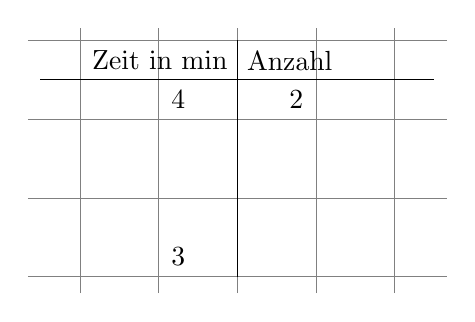
\begin{tikzpicture}[show background grid]
\draw[black] (0cm,0cm) -- (0cm,-3cm); 
\draw[black] (-2.5 cm,-0.5cm) -- (2.5cm,-0.5cm); 
\node[left] at (0 cm,-0.25cm) {Zeit in min};
\node[right] at (0 cm,-0.255cm) {Anzahl};
\node[circle] (1) at (-0.75 cm,-0.75cm) {4};
\node[circle] (2) at (-0.75 cm,-1.75cm) {};
\node[circle] (3) at (-0.75 cm,-2.75cm) {3};
\node[circle] (4) at (0.75 cm,-0.75cm) {2};
\node[circle] (5) at (0.75 cm,-1.75cm) {};
\node[circle] (6) at (0.75 cm,-2.75cm) {};
\end{tikzpicture}
\\\hline
c)&\tikzstyle{background grid}=[draw, black!15,step=.5cm]
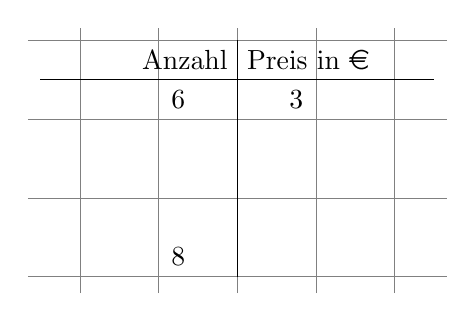
\begin{tikzpicture}[show background grid]
\draw[black] (0cm,0cm) -- (0cm,-3cm); 
\draw[black] (-2.5 cm,-0.5cm) -- (2.5cm,-0.5cm); 
\node[left] at (0 cm,-0.25cm) {Anzahl};
\node[right] at (0 cm,-0.255cm) {Preis in \euro{}};
\node[circle] (1) at (-0.75 cm,-0.75cm) {6};
\node[circle] (2) at (-0.75 cm,-1.75cm) {};
\node[circle] (3) at (-0.75 cm,-2.75cm) {8};
\node[circle] (4) at (0.75 cm,-0.75cm) {3};
\node[circle] (5) at (0.75 cm,-1.75cm) {};
\node[circle] (6) at (0.75 cm,-2.75cm) {};
\end{tikzpicture}
&
d)&\tikzstyle{background grid}=[draw, black!15,step=.5cm]
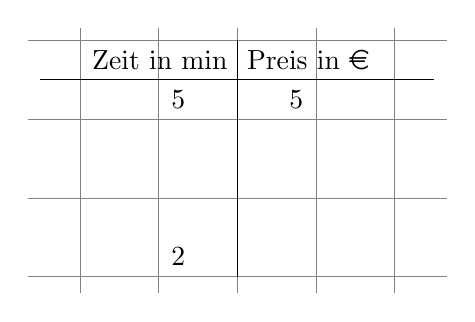
\begin{tikzpicture}[show background grid]
\draw[black] (0cm,0cm) -- (0cm,-3cm); 
\draw[black] (-2.5 cm,-0.5cm) -- (2.5cm,-0.5cm); 
\node[left] at (0 cm,-0.25cm) {Zeit in min};
\node[right] at (0 cm,-0.255cm) {Preis in \euro{}};
\node[circle] (1) at (-0.75 cm,-0.75cm) {5};
\node[circle] (2) at (-0.75 cm,-1.75cm) {};
\node[circle] (3) at (-0.75 cm,-2.75cm) {2};
\node[circle] (4) at (0.75 cm,-0.75cm) {5};
\node[circle] (5) at (0.75 cm,-1.75cm) {};
\node[circle] (6) at (0.75 cm,-2.75cm) {};
\end{tikzpicture}
\\\hline
e)&\tikzstyle{background grid}=[draw, black!15,step=.5cm]
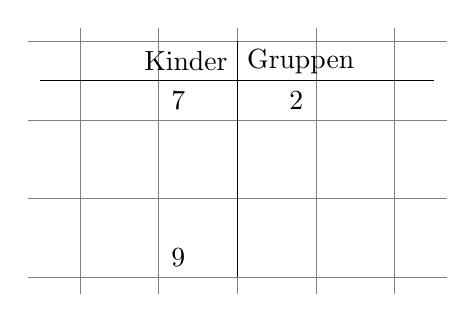
\begin{tikzpicture}[show background grid]
\draw[black] (0cm,0cm) -- (0cm,-3cm); 
\draw[black] (-2.5 cm,-0.5cm) -- (2.5cm,-0.5cm); 
\node[left] at (0 cm,-0.25cm) {Kinder};
\node[right] at (0 cm,-0.255cm) {Gruppen};
\node[circle] (1) at (-0.75 cm,-0.75cm) {7};
\node[circle] (2) at (-0.75 cm,-1.75cm) {};
\node[circle] (3) at (-0.75 cm,-2.75cm) {9};
\node[circle] (4) at (0.75 cm,-0.75cm) {2};
\node[circle] (5) at (0.75 cm,-1.75cm) {};
\node[circle] (6) at (0.75 cm,-2.75cm) {};
\end{tikzpicture}
&
f)&\tikzstyle{background grid}=[draw, black!15,step=.5cm]
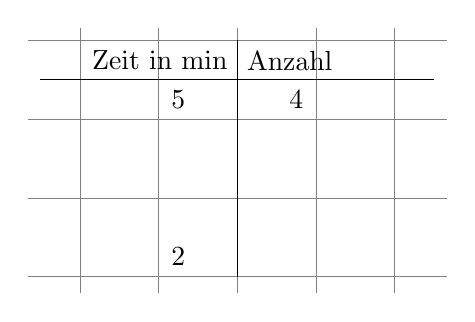
\begin{tikzpicture}[show background grid]
\draw[black] (0cm,0cm) -- (0cm,-3cm); 
\draw[black] (-2.5 cm,-0.5cm) -- (2.5cm,-0.5cm); 
\node[left] at (0 cm,-0.25cm) {Zeit in min};
\node[right] at (0 cm,-0.255cm) {Anzahl};
\node[circle] (1) at (-0.75 cm,-0.75cm) {5};
\node[circle] (2) at (-0.75 cm,-1.75cm) {};
\node[circle] (3) at (-0.75 cm,-2.75cm) {2};
\node[circle] (4) at (0.75 cm,-0.75cm) {4};
\node[circle] (5) at (0.75 cm,-1.75cm) {};
\node[circle] (6) at (0.75 cm,-2.75cm) {};
\end{tikzpicture}
\\\hline
g)&\tikzstyle{background grid}=[draw, black!15,step=.5cm]
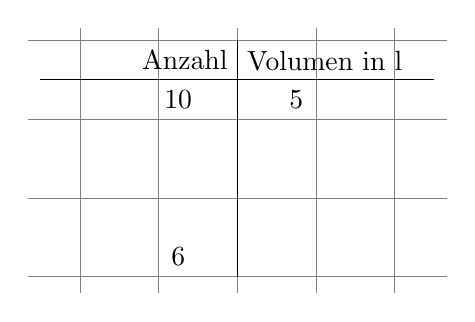
\begin{tikzpicture}[show background grid]
\draw[black] (0cm,0cm) -- (0cm,-3cm); 
\draw[black] (-2.5 cm,-0.5cm) -- (2.5cm,-0.5cm); 
\node[left] at (0 cm,-0.25cm) {Anzahl};
\node[right] at (0 cm,-0.255cm) {Volumen in l};
\node[circle] (1) at (-0.75 cm,-0.75cm) {10};
\node[circle] (2) at (-0.75 cm,-1.75cm) {};
\node[circle] (3) at (-0.75 cm,-2.75cm) {6};
\node[circle] (4) at (0.75 cm,-0.75cm) {5};
\node[circle] (5) at (0.75 cm,-1.75cm) {};
\node[circle] (6) at (0.75 cm,-2.75cm) {};
\end{tikzpicture}
&
h)&\tikzstyle{background grid}=[draw, black!15,step=.5cm]
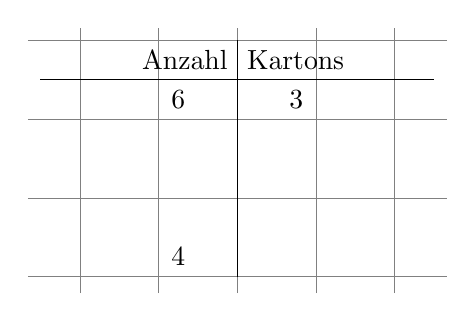
\begin{tikzpicture}[show background grid]
\draw[black] (0cm,0cm) -- (0cm,-3cm); 
\draw[black] (-2.5 cm,-0.5cm) -- (2.5cm,-0.5cm); 
\node[left] at (0 cm,-0.25cm) {Anzahl};
\node[right] at (0 cm,-0.255cm) {Kartons};
\node[circle] (1) at (-0.75 cm,-0.75cm) {6};
\node[circle] (2) at (-0.75 cm,-1.75cm) {};
\node[circle] (3) at (-0.75 cm,-2.75cm) {4};
\node[circle] (4) at (0.75 cm,-0.75cm) {3};
\node[circle] (5) at (0.75 cm,-1.75cm) {};
\node[circle] (6) at (0.75 cm,-2.75cm) {};
\end{tikzpicture}
\\\hline
i)&\tikzstyle{background grid}=[draw, black!15,step=.5cm]
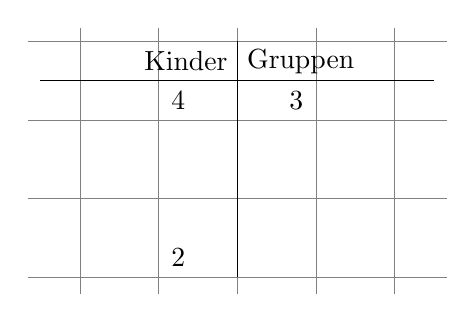
\begin{tikzpicture}[show background grid]
\draw[black] (0cm,0cm) -- (0cm,-3cm); 
\draw[black] (-2.5 cm,-0.5cm) -- (2.5cm,-0.5cm); 
\node[left] at (0 cm,-0.25cm) {Kinder};
\node[right] at (0 cm,-0.255cm) {Gruppen};
\node[circle] (1) at (-0.75 cm,-0.75cm) {4};
\node[circle] (2) at (-0.75 cm,-1.75cm) {};
\node[circle] (3) at (-0.75 cm,-2.75cm) {2};
\node[circle] (4) at (0.75 cm,-0.75cm) {3};
\node[circle] (5) at (0.75 cm,-1.75cm) {};
\node[circle] (6) at (0.75 cm,-2.75cm) {};
\end{tikzpicture}
&
j)&\tikzstyle{background grid}=[draw, black!15,step=.5cm]
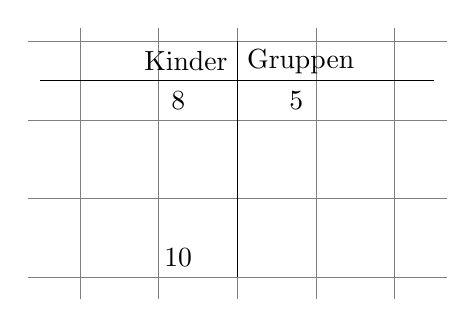
\begin{tikzpicture}[show background grid]
\draw[black] (0cm,0cm) -- (0cm,-3cm); 
\draw[black] (-2.5 cm,-0.5cm) -- (2.5cm,-0.5cm); 
\node[left] at (0 cm,-0.25cm) {Kinder};
\node[right] at (0 cm,-0.255cm) {Gruppen};
\node[circle] (1) at (-0.75 cm,-0.75cm) {8};
\node[circle] (2) at (-0.75 cm,-1.75cm) {};
\node[circle] (3) at (-0.75 cm,-2.75cm) {10};
\node[circle] (4) at (0.75 cm,-0.75cm) {5};
\node[circle] (5) at (0.75 cm,-1.75cm) {};
\node[circle] (6) at (0.75 cm,-2.75cm) {};
\end{tikzpicture}
\\\hline
\end{tabularx}
\vspace{0.5cm}
\newpage
\rightline{Datum: 11.01.2023}
\centerline{{\large Lösungen Hausaufgabentag}} 
\vspace{0.5cm}

\begin{tabularx}{\textwidth}{|C{1.0cm}|X|C{1.0cm}|X|}
\arrayrulecolor{black}\hline
a)&{\tikzstyle{background grid}=[draw, black!15,step=.5cm]
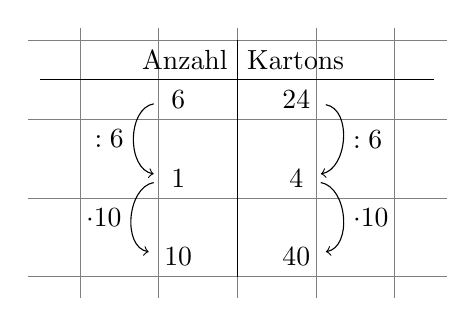
\begin{tikzpicture}[show background grid]
\draw[black] (0cm,0cm) -- (0cm,-3cm); 
\draw[black] (-2.5 cm,-0.5cm) -- (2.5cm,-0.5cm); 
\node[left] at (0 cm,-0.25cm) {Anzahl};
\node[right] at (0 cm,-0.255cm) {Kartons};
\node[circle] (1) at (-0.75 cm,-0.75cm) {6};
\node[circle] (2) at (-0.75 cm,-1.75cm) {1};
\node[circle] (3) at (-0.75 cm,-2.75cm) {10};
\node[circle] (4) at (0.75 cm,-0.75cm) {24};
\node[circle] (5) at (0.75 cm,-1.75cm) {4};
\node[circle] (6) at (0.75 cm,-2.75cm) {40};
\draw[->] (1) to [out=190,in=170] node[left] {$:6$}  (2) ;
\draw[->] (2) to [out=190,in=170] node[left] {$\cdot 10$}  (3) ;
\draw[->] (4) to [out=350,in=10] node[right] {$:6$}  (5) ;
\draw[->] (5) to [out=350,in=10] node[right] {$\cdot 10$}  (6) ;
\end{tikzpicture}}
&
b)&{\tikzstyle{background grid}=[draw, black!15,step=.5cm]
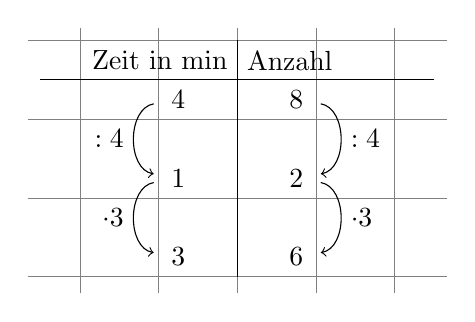
\begin{tikzpicture}[show background grid]
\draw[black] (0cm,0cm) -- (0cm,-3cm); 
\draw[black] (-2.5 cm,-0.5cm) -- (2.5cm,-0.5cm); 
\node[left] at (0 cm,-0.25cm) {Zeit in min};
\node[right] at (0 cm,-0.255cm) {Anzahl};
\node[circle] (1) at (-0.75 cm,-0.75cm) {4};
\node[circle] (2) at (-0.75 cm,-1.75cm) {1};
\node[circle] (3) at (-0.75 cm,-2.75cm) {3};
\node[circle] (4) at (0.75 cm,-0.75cm) {8};
\node[circle] (5) at (0.75 cm,-1.75cm) {2};
\node[circle] (6) at (0.75 cm,-2.75cm) {6};
\draw[->] (1) to [out=190,in=170] node[left] {$:4$}  (2) ;
\draw[->] (2) to [out=190,in=170] node[left] {$\cdot 3$}  (3) ;
\draw[->] (4) to [out=350,in=10] node[right] {$:4$}  (5) ;
\draw[->] (5) to [out=350,in=10] node[right] {$\cdot 3$}  (6) ;
\end{tikzpicture}}
\\\hline
\end{tabularx}
\vspace{0.5cm}
\begin{tabularx}{\textwidth}{|C{1.0cm}|X|C{1.0cm}|X|}
\arrayrulecolor{black}\hline
c)&{\tikzstyle{background grid}=[draw, black!15,step=.5cm]
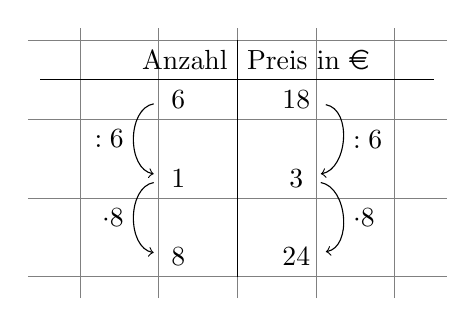
\begin{tikzpicture}[show background grid]
\draw[black] (0cm,0cm) -- (0cm,-3cm); 
\draw[black] (-2.5 cm,-0.5cm) -- (2.5cm,-0.5cm); 
\node[left] at (0 cm,-0.25cm) {Anzahl};
\node[right] at (0 cm,-0.255cm) {Preis in \euro{}};
\node[circle] (1) at (-0.75 cm,-0.75cm) {6};
\node[circle] (2) at (-0.75 cm,-1.75cm) {1};
\node[circle] (3) at (-0.75 cm,-2.75cm) {8};
\node[circle] (4) at (0.75 cm,-0.75cm) {18};
\node[circle] (5) at (0.75 cm,-1.75cm) {3};
\node[circle] (6) at (0.75 cm,-2.75cm) {24};
\draw[->] (1) to [out=190,in=170] node[left] {$:6$}  (2) ;
\draw[->] (2) to [out=190,in=170] node[left] {$\cdot 8$}  (3) ;
\draw[->] (4) to [out=350,in=10] node[right] {$:6$}  (5) ;
\draw[->] (5) to [out=350,in=10] node[right] {$\cdot 8$}  (6) ;
\end{tikzpicture}}
&
d)&{\tikzstyle{background grid}=[draw, black!15,step=.5cm]
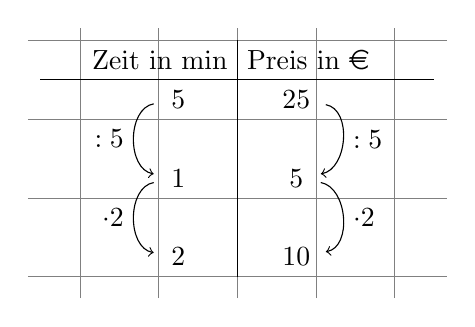
\begin{tikzpicture}[show background grid]
\draw[black] (0cm,0cm) -- (0cm,-3cm); 
\draw[black] (-2.5 cm,-0.5cm) -- (2.5cm,-0.5cm); 
\node[left] at (0 cm,-0.25cm) {Zeit in min};
\node[right] at (0 cm,-0.255cm) {Preis in \euro{}};
\node[circle] (1) at (-0.75 cm,-0.75cm) {5};
\node[circle] (2) at (-0.75 cm,-1.75cm) {1};
\node[circle] (3) at (-0.75 cm,-2.75cm) {2};
\node[circle] (4) at (0.75 cm,-0.75cm) {25};
\node[circle] (5) at (0.75 cm,-1.75cm) {5};
\node[circle] (6) at (0.75 cm,-2.75cm) {10};
\draw[->] (1) to [out=190,in=170] node[left] {$:5$}  (2) ;
\draw[->] (2) to [out=190,in=170] node[left] {$\cdot 2$}  (3) ;
\draw[->] (4) to [out=350,in=10] node[right] {$:5$}  (5) ;
\draw[->] (5) to [out=350,in=10] node[right] {$\cdot 2$}  (6) ;
\end{tikzpicture}}
\\\hline
\end{tabularx}
\vspace{0.5cm}
\begin{tabularx}{\textwidth}{|C{1.0cm}|X|C{1.0cm}|X|}
\arrayrulecolor{black}\hline
e)&{\tikzstyle{background grid}=[draw, black!15,step=.5cm]
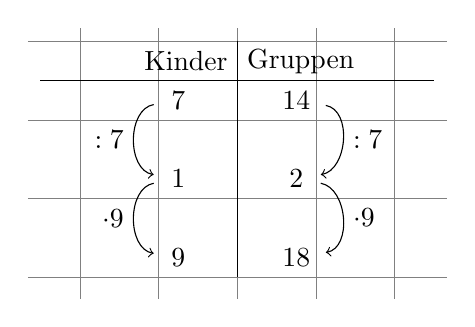
\begin{tikzpicture}[show background grid]
\draw[black] (0cm,0cm) -- (0cm,-3cm); 
\draw[black] (-2.5 cm,-0.5cm) -- (2.5cm,-0.5cm); 
\node[left] at (0 cm,-0.25cm) {Kinder};
\node[right] at (0 cm,-0.255cm) {Gruppen};
\node[circle] (1) at (-0.75 cm,-0.75cm) {7};
\node[circle] (2) at (-0.75 cm,-1.75cm) {1};
\node[circle] (3) at (-0.75 cm,-2.75cm) {9};
\node[circle] (4) at (0.75 cm,-0.75cm) {14};
\node[circle] (5) at (0.75 cm,-1.75cm) {2};
\node[circle] (6) at (0.75 cm,-2.75cm) {18};
\draw[->] (1) to [out=190,in=170] node[left] {$:7$}  (2) ;
\draw[->] (2) to [out=190,in=170] node[left] {$\cdot 9$}  (3) ;
\draw[->] (4) to [out=350,in=10] node[right] {$:7$}  (5) ;
\draw[->] (5) to [out=350,in=10] node[right] {$\cdot 9$}  (6) ;
\end{tikzpicture}}
&
f)&{\tikzstyle{background grid}=[draw, black!15,step=.5cm]
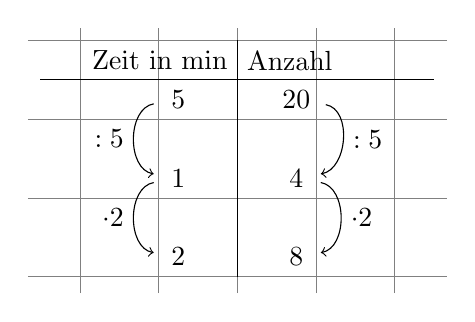
\begin{tikzpicture}[show background grid]
\draw[black] (0cm,0cm) -- (0cm,-3cm); 
\draw[black] (-2.5 cm,-0.5cm) -- (2.5cm,-0.5cm); 
\node[left] at (0 cm,-0.25cm) {Zeit in min};
\node[right] at (0 cm,-0.255cm) {Anzahl};
\node[circle] (1) at (-0.75 cm,-0.75cm) {5};
\node[circle] (2) at (-0.75 cm,-1.75cm) {1};
\node[circle] (3) at (-0.75 cm,-2.75cm) {2};
\node[circle] (4) at (0.75 cm,-0.75cm) {20};
\node[circle] (5) at (0.75 cm,-1.75cm) {4};
\node[circle] (6) at (0.75 cm,-2.75cm) {8};
\draw[->] (1) to [out=190,in=170] node[left] {$:5$}  (2) ;
\draw[->] (2) to [out=190,in=170] node[left] {$\cdot 2$}  (3) ;
\draw[->] (4) to [out=350,in=10] node[right] {$:5$}  (5) ;
\draw[->] (5) to [out=350,in=10] node[right] {$\cdot 2$}  (6) ;
\end{tikzpicture}}
\\\hline
\end{tabularx}
\vspace{0.5cm}
\begin{tabularx}{\textwidth}{|C{1.0cm}|X|C{1.0cm}|X|}
\arrayrulecolor{black}\hline
g)&{\tikzstyle{background grid}=[draw, black!15,step=.5cm]
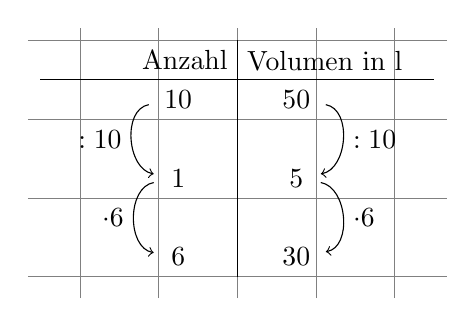
\begin{tikzpicture}[show background grid]
\draw[black] (0cm,0cm) -- (0cm,-3cm); 
\draw[black] (-2.5 cm,-0.5cm) -- (2.5cm,-0.5cm); 
\node[left] at (0 cm,-0.25cm) {Anzahl};
\node[right] at (0 cm,-0.255cm) {Volumen in l};
\node[circle] (1) at (-0.75 cm,-0.75cm) {10};
\node[circle] (2) at (-0.75 cm,-1.75cm) {1};
\node[circle] (3) at (-0.75 cm,-2.75cm) {6};
\node[circle] (4) at (0.75 cm,-0.75cm) {50};
\node[circle] (5) at (0.75 cm,-1.75cm) {5};
\node[circle] (6) at (0.75 cm,-2.75cm) {30};
\draw[->] (1) to [out=190,in=170] node[left] {$:10$}  (2) ;
\draw[->] (2) to [out=190,in=170] node[left] {$\cdot 6$}  (3) ;
\draw[->] (4) to [out=350,in=10] node[right] {$:10$}  (5) ;
\draw[->] (5) to [out=350,in=10] node[right] {$\cdot 6$}  (6) ;
\end{tikzpicture}}
&
h)&{\tikzstyle{background grid}=[draw, black!15,step=.5cm]
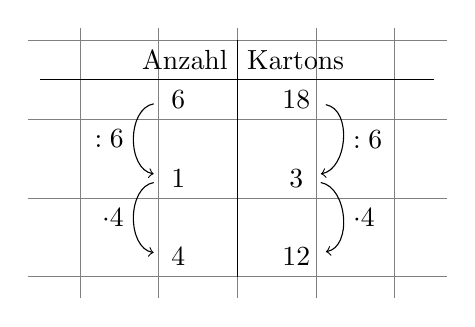
\begin{tikzpicture}[show background grid]
\draw[black] (0cm,0cm) -- (0cm,-3cm); 
\draw[black] (-2.5 cm,-0.5cm) -- (2.5cm,-0.5cm); 
\node[left] at (0 cm,-0.25cm) {Anzahl};
\node[right] at (0 cm,-0.255cm) {Kartons};
\node[circle] (1) at (-0.75 cm,-0.75cm) {6};
\node[circle] (2) at (-0.75 cm,-1.75cm) {1};
\node[circle] (3) at (-0.75 cm,-2.75cm) {4};
\node[circle] (4) at (0.75 cm,-0.75cm) {18};
\node[circle] (5) at (0.75 cm,-1.75cm) {3};
\node[circle] (6) at (0.75 cm,-2.75cm) {12};
\draw[->] (1) to [out=190,in=170] node[left] {$:6$}  (2) ;
\draw[->] (2) to [out=190,in=170] node[left] {$\cdot 4$}  (3) ;
\draw[->] (4) to [out=350,in=10] node[right] {$:6$}  (5) ;
\draw[->] (5) to [out=350,in=10] node[right] {$\cdot 4$}  (6) ;
\end{tikzpicture}}
\\\hline
\end{tabularx}
\vspace{0.5cm}
\begin{tabularx}{\textwidth}{|C{1.0cm}|X|C{1.0cm}|X|}
\arrayrulecolor{black}\hline
i)&{\tikzstyle{background grid}=[draw, black!15,step=.5cm]
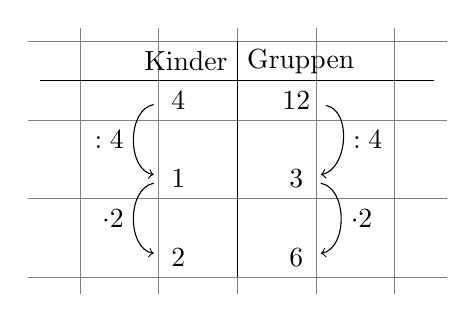
\begin{tikzpicture}[show background grid]
\draw[black] (0cm,0cm) -- (0cm,-3cm); 
\draw[black] (-2.5 cm,-0.5cm) -- (2.5cm,-0.5cm); 
\node[left] at (0 cm,-0.25cm) {Kinder};
\node[right] at (0 cm,-0.255cm) {Gruppen};
\node[circle] (1) at (-0.75 cm,-0.75cm) {4};
\node[circle] (2) at (-0.75 cm,-1.75cm) {1};
\node[circle] (3) at (-0.75 cm,-2.75cm) {2};
\node[circle] (4) at (0.75 cm,-0.75cm) {12};
\node[circle] (5) at (0.75 cm,-1.75cm) {3};
\node[circle] (6) at (0.75 cm,-2.75cm) {6};
\draw[->] (1) to [out=190,in=170] node[left] {$:4$}  (2) ;
\draw[->] (2) to [out=190,in=170] node[left] {$\cdot 2$}  (3) ;
\draw[->] (4) to [out=350,in=10] node[right] {$:4$}  (5) ;
\draw[->] (5) to [out=350,in=10] node[right] {$\cdot 2$}  (6) ;
\end{tikzpicture}}
&
j)&{\tikzstyle{background grid}=[draw, black!15,step=.5cm]
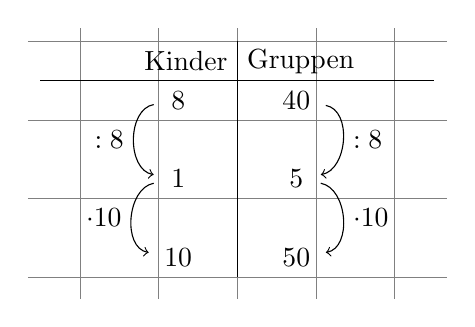
\begin{tikzpicture}[show background grid]
\draw[black] (0cm,0cm) -- (0cm,-3cm); 
\draw[black] (-2.5 cm,-0.5cm) -- (2.5cm,-0.5cm); 
\node[left] at (0 cm,-0.25cm) {Kinder};
\node[right] at (0 cm,-0.255cm) {Gruppen};
\node[circle] (1) at (-0.75 cm,-0.75cm) {8};
\node[circle] (2) at (-0.75 cm,-1.75cm) {1};
\node[circle] (3) at (-0.75 cm,-2.75cm) {10};
\node[circle] (4) at (0.75 cm,-0.75cm) {40};
\node[circle] (5) at (0.75 cm,-1.75cm) {5};
\node[circle] (6) at (0.75 cm,-2.75cm) {50};
\draw[->] (1) to [out=190,in=170] node[left] {$:8$}  (2) ;
\draw[->] (2) to [out=190,in=170] node[left] {$\cdot 10$}  (3) ;
\draw[->] (4) to [out=350,in=10] node[right] {$:8$}  (5) ;
\draw[->] (5) to [out=350,in=10] node[right] {$\cdot 10$}  (6) ;
\end{tikzpicture}}
\\\hline
\end{tabularx}
\vspace{0.5cm}
\begin{tabularx}{\textwidth}{|C{1.0cm}|X|C{1.0cm}|X|}
\arrayrulecolor{black}\hline
\end{tabularx}
\vspace{0.5cm}
\end{document}